
\documentclass{article} % For LaTeX2e
\usepackage[submission]{colm2025_conference}

\usepackage{microtype}
\usepackage{hyperref}
\usepackage{url}
\usepackage{booktabs}

\usepackage{lineno}
\usepackage{graphicx}
\usepackage{tcolorbox}
\usepackage{tikz}
\usetikzlibrary{positioning, fit, arrows.meta, shapes.geometric}
\usepackage{wrapfig}

\definecolor{darkblue}{rgb}{0, 0, 0.5}
\hypersetup{colorlinks=true, citecolor=darkblue, linkcolor=darkblue, urlcolor=darkblue}


\title{AutoLibra \protect
\includegraphics[height=1em]{figs/scale.png} \\ \textit{Metric Induction from Open-Ended Human Input for Agents}}

% Authors must not appear in the submitted version. They should be hidden
% as long as the \colmfinalcopy macro remains commented out below.
% Non-anonymous submissions will be rejected without review.

\author{Antiquus S.~Hippocampus, Natalia Cerebro \& Amelie P. Amygdale \thanks{ Use footnote for providing further information
about author (webpage, alternative address)---\emph{not} for acknowledging
funding agencies.  Funding acknowledgements go at the end of the paper.} \\
Department of Computer Science\\
Cranberry-Lemon University\\
Pittsburgh, PA 15213, USA \\
\texttt{\{hippo,brain,jen\}@cs.cranberry-lemon.edu} \\
\And
Ji Q. Ren \& Yevgeny LeNet \\
Department of Computational Neuroscience \\
University of the Witwatersrand \\
Joburg, South Africa \\
\texttt{\{robot,net\}@wits.ac.za} \\
\AND
Coauthor \\
Affiliation \\
Address \\
\texttt{email}
}

% The \author macro works with any number of authors. There are two commands
% used to separate the names and addresses of multiple authors: \And and \AND.
%
% Using \And between authors leaves it to \LaTeX{} to determine where to break
% the lines. Using \AND forces a linebreak at that point. So, if \LaTeX{}
% puts 3 of 4 authors names on the first line, and the last on the second
% line, try using \AND instead of \And before the third author name.

\newcommand{\fix}{\marginpar{FIX}}
\newcommand{\new}{\marginpar{NEW}}

\begin{document}

\ifcolmsubmission
\linenumbers
\fi

\maketitle

\begin{abstract}
The evaluation and optimization of language agents are often based on either
task success or heuristically designed metrics.
However, these approaches are either not fine-grained enough or require 
manual design of the metrics by experts.
We propose \emph{AutoLibra},
a system that transforms human feedback, 
\emph{e.g.} ``\textsf{If you find that the button is disabled, don't click it again}'',
or ``\textsf{This agent has too much autonomy to decide what to do on its own}''
into metrics evaluating similar failure and successful modes.
AutoLibra accomplishes this by first grounding the feedback in the agent's behavior,
clustering similar positive and negative behaviors,
and creating metrics that are ready to prompt LLM-as-a-Judge with
concrete examples and definitions. 
We propose two \emph{meta metrics} to evaluate how aligned a set of (induced) metrics
is with human open-ended feedback: ``coverage'' and ``redundancy''.
Through optimizing these meta metrics, we find that AutoLibra could
not only recover the \textbf{agent evaluation} dimensions heuristically proposed
in previous agent evaluation benchmarks, but also discover the ones that have been overlooked.
Beyond agent evaluation, we demonstrate two practical applications of
AutoLibra in \textbf{agent improvement}:
First, we show that AutoLibra effectively selects high-quality agent fine-tuning data
for web browsing. Second, we demonstrate that the metrics extracted by AutoLibra serve
as better optimization targets than task success rate on two challenging text game tasks,
enhancing prompt engineering.
Our results suggest that AutoLibra can use very small number of annotations (less than 100 annotations), 
to induce a set of interpretable metrics with higher than 80\% coverage on unseen feedback.
\end{abstract}


\section{Introduction}

\begin{wrapfigure}{r}{0.5\textwidth}
   \vspace{-45pt}
   \centering
   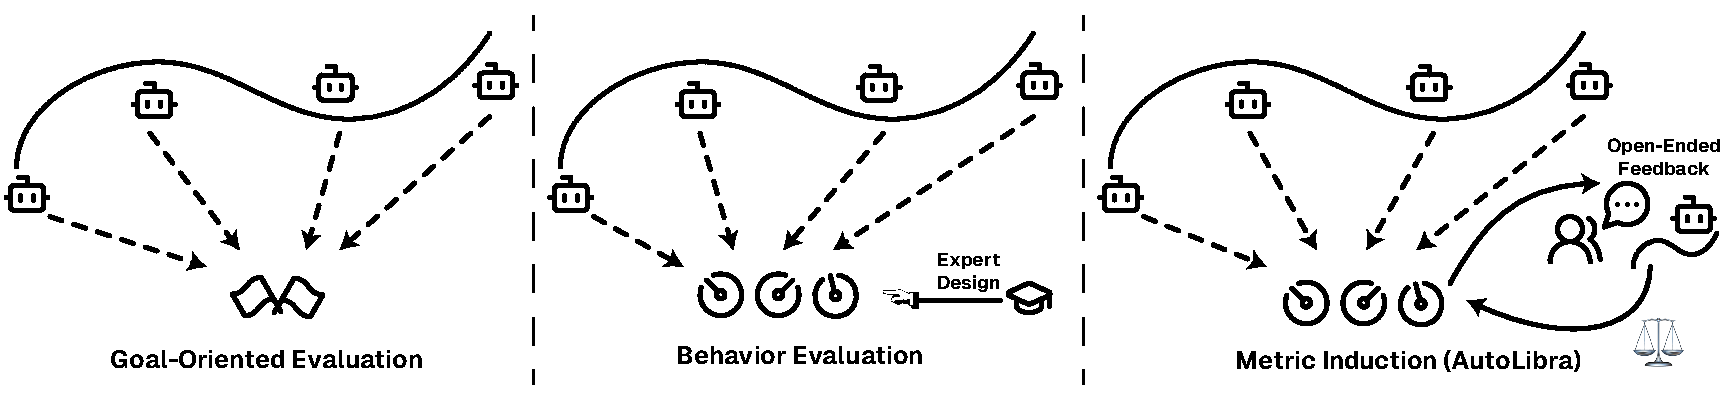
\includegraphics[width=0.5\textwidth]{figs/autolibra.pdf}
   \caption{Comparison of AutoLibra with existing agent evaluation paradigms.}
\end{wrapfigure}


In the development process, humans receive feedback from others,
both praises and critics, although not all are accurate or constructive.
We summarize and internalize the feedback into
generalizable self-evaluation metrics. Compared to the scarce reward
we get from achieving goals, these metrics offer a lens for self-reflection on the
strengths and weaknesses of ourselves and a ladder for self-improvement.
In this paper, we ask:
\textbf{can we automatically induce metrics to evaluate and improve language agents from natural language feedback?} 

   
The current evaluation of large language model (LLM) agents and reward modeling often fall
into two paradigms: (1) goal-oriented evaluation --
\emph{whether the agents have fulfilled the given task},
\emph{e.g.} \citet{zhouwebarena,jimenezswe,chan2024mle,paglieri2024balrog}
and (2) behavior evaluation -- \emph{how well the agents do on heuristically designed dimensions},
\emph{e.g.} \citet{zhousotopia,shao2024collaborative,pan2025why}. 
Goal-oriented evaluation is often verifiable, but it is not fine-grained or comprehensive enough
to diagnose agents' behavior problems or find the bottlenecks for improvements. 
While behavior evaluation complements it, it requires manual design of the metrics by experts,
which is time-consuming, may not align with users' opinions, and often not concrete enough. 

We introduce AutoLibra \protect
\includegraphics[height=1em]{figs/scale.png}, an automatic metric induction method,
as a new paradigm for agent evaluation and improvement.
This method offers behavior evaluation for agents, while (1) automating the metric creation process with LLMs, 
(2) optimizing the alignment through searching for a set of metrics to cover human feedback with minimal redundancy,
and (3) providing concrete examples of good and bad behaviors for each metric to improve the
LLM-as-a-Judge's performance. 

AutoLibra takes in agent trajectories along with human open-ended feedback, and generates a set of metrics, each with a name, description, and a list of good behavior examples, and bad behavior examples. AutoLibra 



\begin{wrapfigure}{r}{0.7\textwidth}
    \centering
    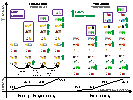
\includegraphics[width=0.7\textwidth]{figs/autolibra-teaser.pdf}
    \caption{Caption}
    \label{fig:enter-label}
\end{wrapfigure}

\section{AutoLibra\protect
\includegraphics[height=1em]{figs/scale.png}}


\section{The lens \protect
\includegraphics[height=1em]{figs/microscope.png}: Agent evaluation with AutoLibra}
\section{The ladder \protect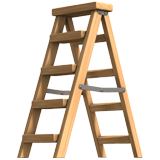
\includegraphics[height=1em]{figs/ladder.png}: Agent improvement with AutoLibra}
\subsection{Style}

Papers to be submitted to COLM 2025 must be prepared according to the
instructions presented here.

%% Please note that we have introduced automatic line number generation
%% into the style file for \LaTeXe. This is to help reviewers
%% refer to specific lines of the paper when they make their comments. Please do
%% NOT refer to these line numbers in your paper as they will be removed from the
%% style file for the final version of accepted papers.

Authors are required to use the COLM \LaTeX{} style files obtainable at the
COLM website. Please make sure you use the current files and
not previous versions. Tweaking the style files may be grounds for rejection.

\subsubsection{Copy Options}

If your paper is ultimately accepted, the option {\tt
  {\textbackslash}final} should be set  for the {\tt {\textbackslash}usepackage[submission]\{colm2025\_conference\}} command for the camera ready version. The {\tt submission} options is the default, and is to be used for all submissions during the review process. It also turns on the line numbers. If you wish to submit a preprint, the option {\tt preprint} should be used.
  
  

\subsection{Retrieval of style files}

The style files for COLM and other conference information are available online at:
\begin{center}
   \url{http://www.colmweb.org/}
\end{center}
The file \verb+colm2025_conference.pdf+ contains these
instructions and illustrates the
various formatting requirements your COLM paper must satisfy.
Submissions must be made using \LaTeX{} and the style files
\verb+colm2025_conference.sty+ and \verb+colm2025_conference.bst+ (to be used with \LaTeX{}2e). The file
\verb+colm2025_conference.tex+ may be used as a ``shell'' for writing your paper. All you
have to do is replace the author, title, abstract, and text of the paper with
your own.

The formatting instructions contained in these style files are summarized in
sections \ref{gen_inst}, \ref{headings}, and \ref{others} below.

\section{General formatting instructions}
\label{gen_inst}

The text must be confined within a rectangle 5.5~inches (33~picas) wide and
9~inches (54~picas) long. The left margin is 1.5~inch (9~picas).
Use 10~point type with a vertical spacing of 11~points. Palatino is the
preferred typeface throughout, and is mandatory for the main text. Paragraphs are separated by 1/2~line space, with no indentation. 

Paper title is 17~point and left-aligned.
All pages should start at 1~inch (6~picas) from the top of the page.

Please verify that any custom header information you may add does not override the style defined in this document. This has been known to occur especially when submissions are converted to a new template from a previous one (i.e., for re-submission to a different venue). 

Authors' names are
set in boldface, and each name is placed above its corresponding
address. The lead author's name is to be listed first, and
the co-authors' names are set to follow. Authors sharing the
same address can be on the same line.

Please pay special attention to the instructions in section \ref{others}
regarding figures, tables, acknowledgements, and references.


There will be a strict upper limit of 9 pages for the main text of the initial submission, with unlimited additional pages for citations. 

We strongly recommend following arXiv's guidelines for making your paper friendly for HTML conversion: \url{https://info.arxiv.org/help/submit_latex_best_practices.html}.


\section{Headings: first level}
\label{headings}

First level headings are in lower case (except for first word and proper nouns), bold face,
flush left and in point size 12. One line space before the first level
heading and 1/2~line space after the first level heading.

\subsection{Headings: second level}

Second level headings are in lower case (except for first word and proper nouns), bold face,
flush left and in point size 10. One line space before the second level
heading and 1/2~line space after the second level heading.

\subsubsection{Headings: third level}

Third level headings are in lower case (except for first word and proper nouns), bold face, italics, 
flush left and in point size 10. One line space before the third level
heading and 1/2~line space after the third level heading.

\section{Citations, figures, tables, references}\label{others}

These instructions apply to everyone, regardless of the formatter being used.

\subsection{Citations within the text}

Citations within the text should be based on the \texttt{natbib} package
and include the authors' last names and year (with the ``et~al.'' construct
for more than two authors). When the authors or the publication are
included in the sentence, the citation should not be in parenthesis using \verb|\citet{}| (as
in ``See \citet{Vaswani+2017} for more information.''). Otherwise, the citation
should be in parenthesis using \verb|\citep{}| (as in ``Transformers are a key tool
for developing language models~\citep{Vaswani+2017}.'').

The corresponding references are to be listed in alphabetical order of
authors, in the \textsc{References} section. As to the format of the
references themselves, any style is acceptable as long as it is used
consistently.

\subsection{Footnotes}

Indicate footnotes with a number\footnote{Sample of the first footnote} in the
text. Place the footnotes at the bottom of the page on which they appear.
Precede the footnote with a horizontal rule of 2~inches
(12~picas).\footnote{Sample of the second footnote}

\subsection{Figures}

All artwork must be neat, clean, and legible. Lines should be dark
enough for purposes of reproduction; art work should not be
hand-drawn. Any text within the figure must be readable. We ask to not use font sizes below {\tt small}. We strongly recommend to use vector representations (e.g., pdf or svg) for all diagrams. 
We strongly recommend positioning all figures at the top or bottom of the page.

The figure number and caption always appear below the figure. Place one line space before the figure caption, and one line space after the figure. The figure caption is lower case (except for first word and proper nouns); figures are numbered consecutively.
Make sure the figure caption does not get separated from the figure.
Leave sufficient space to avoid splitting the figure and figure caption.

You may use color figures.
However, it is best for the
figure captions and the paper body to make sense if the paper is printed
either in black/white or in color.
\begin{figure}[t]
\begin{center}
%\framebox[4.0in]{$\;$}
\fbox{\rule[-.5cm]{0cm}{4cm} \rule[-.5cm]{4cm}{0cm}}
\end{center}
\caption{Sample figure caption.}
\end{figure}

\subsection{Tables}

All tables must be centered, neat, clean and legible. Do not use hand-drawn tables. The table number and title always appear below the table. See Table~\ref{sample-table}. Please do not use font sizes below {\tt small} in tables. We recommend using {\tt booktabs} or a similar package to style tables. 
We strongly recommend positioning all tables at the top or bottom of the page.

Place one line space before the table title, one line space after the table title, and one line space after the table. The table title must be lowercase (except for first word and proper nouns); tables are numbered consecutively.

\begin{table}[t]
\begin{center}
\begin{tabular}{ll}
\toprule
\multicolumn{1}{c}{\bf PART}  &\multicolumn{1}{c}{\bf DESCRIPTION} \\
\midrule
Dendrite         &Input terminal \\
Axon             &Output terminal \\
Soma             &Cell body (contains cell nucleus) \\
\bottomrule
\end{tabular}
\end{center}
\caption{Sample table title}\label{sample-table}
\end{table}




\section{Final instructions}
Do not change any aspects of the formatting parameters in the style files.
In particular, do not modify the width or length of the rectangle the text
should fit into, and do not change font sizes (except perhaps in the
\textsc{References} section; see below). Please note that pages should be
numbered.

\section{Preparing PostScript or PDF files}

Please prepare PostScript or PDF files with paper size ``US Letter'', and
not, for example, ``A4''. The -t
letter option on dvips will produce US Letter files.

Consider directly generating PDF files using \verb+pdflatex+
(especially if you are a MiKTeX user).
PDF figures must be substituted for EPS figures, however.

Otherwise, please generate your PostScript and PDF files with the following commands:
\begin{verbatim}
dvips mypaper.dvi -t letter -Ppdf -G0 -o mypaper.ps
ps2pdf mypaper.ps mypaper.pdf
\end{verbatim}

\subsection{Margins in LaTeX}

Most of the margin problems come from figures positioned by hand using
\verb+\special+ or other commands. We suggest using the command
\verb+\includegraphics+
from the graphicx package. Always specify the figure width as a multiple of
the line width as in the example below using .eps graphics
\begin{verbatim}
   \usepackage[dvips]{graphicx} ...
   \includegraphics[width=0.8\linewidth]{myfile.eps}
\end{verbatim}
or % Apr 2009 addition
\begin{verbatim}
   \usepackage[pdftex]{graphicx} ...
   \includegraphics[width=0.8\linewidth]{myfile.pdf}
\end{verbatim}
for .pdf graphics.
See section~4.4 in the graphics bundle documentation (\url{http://www.ctan.org/tex-archive/macros/latex/required/graphics/grfguide.ps})

A number of width problems arise when LaTeX cannot properly hyphenate a
line. Please give LaTeX hyphenation hints using the \verb+\-+ command.

\section*{Author Contributions}
If you'd like to, you may include  a section for author contributions as is done
in many journals. This is optional and at the discretion of the authors.

\section*{Acknowledgments}
Use unnumbered first level headings for the acknowledgments. All
acknowledgments, including those to funding agencies, go at the end of the paper.

\section*{Ethics Statement}
Authors can add an optional ethics statement to the paper. 
For papers that touch on ethical issues, this section will be evaluated as part of the review process. The ethics statement should come at the end of the paper. It does not count toward the page limit, but should not be more than 1 page. 



\bibliography{colm2025_conference}
\bibliographystyle{colm2025_conference}

\appendix
\section{Appendix}
You may include other additional sections here.

\end{document}
